\documentclass[aos,preprint]{imsart}

% Updated: 2025-06-02
% v0.1: remove \transpose, use T instead 
% v0.2: 

\RequirePackage{amsbsy}       % for \boldsymbol
\RequirePackage{amssymb}      % for \intercal
\RequirePackage{amsopn}       % DeclareMathOperator
\RequirePackage{amsfonts}
\RequirePackage{amsthm}       % theorem
\RequirePackage{physics}      % dd
\RequirePackage{bm}           % bm

\newcommand{\refFig}[1]{Fig.~{\ref{#1}}}
\newcommand{\refEq}[1]{Eq.~{\eqref{#1}}}
\newcommand{\refTab}[1]{Table~{\ref{#1}}}
\newcommand{\refSec}[1]{Section~{\ref{#1}}}
\newcommand{\refLem}[1]{Lemma~{\ref{#1}}}
\newcommand{\refCor}[1]{Corollary~{\ref{#1}}}
\newcommand{\refThm}[1]{Theorem~{\ref{#1}}}
\newcommand{\refProp}[1]{Proposition~{\ref{#1}}}
\newcommand{\refEx}[1]{Example~{\ref{#1}}}
\newcommand{\refDef}[1]{Definition~{\ref{#1}}}
\newcommand{\refApp}[1]{Appendix~{\ref{#1}}}
\newcommand{\refBox}[1]{Box~{\ref{#1}}}


\theoremstyle{plain}
\newtheorem{thm}{Theorem}[section]
\newtheorem*{hoofdstelling}{Claim}
\newtheorem{lemma}[thm]{Lemma}
\newtheorem{prop}[thm]{Proposition}
\newtheorem{eigenschappen}{Properties}
\newtheorem{coro}[thm]{Corollary}
\theoremstyle{definition}
\newtheorem{define}[thm]{Definition}
\newtheorem{example}[thm]{Example}
\newtheorem{remark}[thm]{Remark}
\newtheorem{question}[thm]{Question}
\newtheorem{exercise}{Exercise}[section]

% ==============================================================================
% OPERATORS                                                                    
% ==============================================================================

% use T instead of \transpose
% https://tex.stackexchange.com/questions/587275/the-transpose-correct-or-mostly-agreed-upon-notation-concern
% \makeatletter
% \newcommand*{\transpose}{\bgroup\@transpose}
% \newcommand*{\@transpose}[1][0]{\mathpalette\@@transpose{#1}\egroup}
% \newcommand*{\@@transpose}[2]{\setbox0=\hbox{\m@th$#1\mkern-#2mu\intercal$}\raise\dp0\box0}
% \makeatother

% NEVER RE-define \or and \and used in \author

\DeclareMathOperator*{\argmin}{arg\, min}
\DeclareMathOperator*{\argmax}{arg\, max}
\DeclareMathOperator*{\argsup}{arg\, sup}
\DeclareMathOperator*{\arginf}{arg\, inf}

\newcommand{\conv}{\mathrm{conv}}

\newcommand{\iid}{\; \overset{\mathrm{i.i.d.}}{\sim} \;}

% inspired by texab.sty
\DeclareMathOperator{\PRSymbol}{\mathrm{P}}
\DeclareMathOperator{\ERWSymbol}{\mathbb{E}}

% Defaults: P and E
\newcommand{\PR}[2][\PRSymbol]{#1 \left( {#2} \right)}
\newcommand{\PRi}[3][\PRSymbol]{#1_{#2} \left( {#3} \right)}
\newcommand{\condPR}[3][\PRSymbol]{{#1} \left({#2} \;\middle|\; {#3} \right)}
\newcommand{\condPRi}[4][\PRSymbol]{{#1}_{#2} \left( {#3} \;\middle|\; {#4} \right)}

\newcommand{\ERW}[2][\ERWSymbol]{#1 \left[ {#2} \right]}
\newcommand{\ERWi}[3][\ERWSymbol]{#1_{#2} \left[ {#3} \right]}
\newcommand{\condERW}[3][\ERWSymbol]{#1 \left[ {#2} \cond {#3} \right]}
\newcommand{\condERWi}[4][\ERWSymbol]{{#1}_{#2} \left[ {#3} \;\middle|\; {#4} \right]}

\newcommand{\VAR}[2][\mathrm{Var}]{#1 \left( {#2} \right)}

% <#1, #2>
\newcommand{\spri}[1]{\left\langle {#1} \right\rangle}
\newcommand{\spr}[2]{\left\langle {#1} \, , {#2} \right\rangle}

% ==============================================================================
% LETTERS                                                                      
% ==============================================================================

% boldface
\newcommand{\Af}{\mathbb{A}}
\newcommand{\Bf}{\mathbb{B}}
\newcommand{\Cf}{\mathbb{C}}
\newcommand{\Df}{\mathbb{D}}
\newcommand{\Ef}{\mathbb{E}}
\newcommand{\Ff}{\mathbb{F}}
\newcommand{\Gf}{\mathbb{G}}
\newcommand{\Hf}{\mathbb{H}}
% \newcommand{\If}{\mathbb{I}} % conflict with \If
\newcommand{\Jf}{\mathbb{J}}
\newcommand{\Kf}{\mathbb{K}}
\newcommand{\Lf}{\mathbb{L}}
\newcommand{\Mf}{\mathbb{M}}
\newcommand{\Nf}{\mathbb{N}}
\newcommand{\Of}{\mathbb{O}}
\newcommand{\Pf}{\mathbb{P}}
\newcommand{\Qf}{\mathbb{Q}}
\newcommand{\Rf}{\mathbb{R}}
\newcommand{\Sf}{\mathbb{S}}
\newcommand{\Tf}{\mathbb{T}}
\newcommand{\Uf}{\mathbb{U}}
\newcommand{\Vf}{\mathbb{V}}
\newcommand{\Wf}{\mathbb{W}}
\newcommand{\Xf}{\mathbb{X}}
\newcommand{\Yf}{\mathbb{Y}}
\newcommand{\Zf}{\mathbb{Z}}

% calligraphic
\newcommand{\Ac}{\mathcal{A}}
\newcommand{\Bc}{\mathcal{B}}
\newcommand{\Cc}{\mathcal{C}}
\newcommand{\Dc}{\mathcal{D}}
\newcommand{\Ec}{\mathcal{E}}
\newcommand{\Fc}{\mathcal{F}}
\newcommand{\Gc}{\mathcal{G}}
\newcommand{\Hc}{\mathcal{H}}
\newcommand{\Ic}{\mathcal{I}}
\newcommand{\Jc}{\mathcal{J}}
\newcommand{\Kc}{\mathcal{K}}
\newcommand{\Lc}{\mathcal{L}}
\newcommand{\Mc}{\mathcal{M}}
\newcommand{\Nc}{\mathcal{N}}
\newcommand{\Oc}{\mathcal{O}}
\newcommand{\Pc}{\mathcal{P}}
\newcommand{\Qc}{\mathcal{Q}}
\newcommand{\Rc}{\mathcal{R}}
\newcommand{\Sc}{\mathcal{S}}
\newcommand{\Tc}{\mathcal{T}}
\newcommand{\Uc}{\mathcal{U}}
\newcommand{\Vc}{\mathcal{V}}
\newcommand{\Wc}{\mathcal{W}}
\newcommand{\Xc}{\mathcal{X}}
\newcommand{\Yc}{\mathcal{Y}}
\newcommand{\Zc}{\mathcal{Z}}

% fraktur
\newcommand{\Ak}{\mathfrak{A}}
\newcommand{\Bk}{\mathfrak{B}}
\newcommand{\Ck}{\mathfrak{C}}
\newcommand{\Dk}{\mathfrak{D}}
\newcommand{\Ek}{\mathfrak{E}}
\newcommand{\Fk}{\mathfrak{F}}
\newcommand{\Gk}{\mathfrak{G}}
\newcommand{\Hk}{\mathfrak{H}}
\newcommand{\Ik}{\mathfrak{I}}
\newcommand{\Jk}{\mathfrak{J}}
\newcommand{\Kk}{\mathfrak{K}}
\newcommand{\Lk}{\mathfrak{L}}
\newcommand{\Mk}{\mathfrak{M}}
\newcommand{\Nk}{\mathfrak{N}}
\newcommand{\Ok}{\mathfrak{O}}
\newcommand{\Pk}{\mathfrak{P}}
\newcommand{\Qk}{\mathfrak{Q}}
\newcommand{\Rk}{\mathfrak{R}}
\newcommand{\Sk}{\mathfrak{S}}
\newcommand{\Tk}{\mathfrak{T}}
\newcommand{\Uk}{\mathfrak{U}}
\newcommand{\Vk}{\mathfrak{V}}
\newcommand{\Wk}{\mathfrak{W}}
\newcommand{\Xk}{\mathfrak{X}}
\newcommand{\Yk}{\mathfrak{Y}}
\newcommand{\Zk}{\mathfrak{Z}}

% mathtt
\newcommand{\At}{\mathtt{A}}
\newcommand{\Bt}{\mathtt{B}}
\newcommand{\Ct}{\mathtt{C}}
\newcommand{\Dt}{\mathtt{D}}
\newcommand{\Et}{\mathtt{E}}
\newcommand{\Ft}{\mathtt{F}}
\newcommand{\Gt}{\mathtt{G}}
\newcommand{\Ht}{\mathtt{H}}
\newcommand{\It}{\mathtt{I}}
\newcommand{\Jt}{\mathtt{J}}
\newcommand{\Kt}{\mathtt{K}}
\newcommand{\Lt}{\mathtt{L}}
\newcommand{\Mt}{\mathtt{M}}
\newcommand{\Nt}{\mathtt{N}}
\newcommand{\Ot}{\mathtt{O}}
\newcommand{\Pt}{\mathtt{P}}
\newcommand{\Qt}{\mathtt{Q}}
\newcommand{\Rt}{\mathtt{R}}
\newcommand{\St}{\mathtt{S}}
\newcommand{\Tt}{\mathtt{T}}
\newcommand{\Ut}{\mathtt{U}}
\newcommand{\Vt}{\mathtt{V}}
\newcommand{\Wt}{\mathtt{W}}
\newcommand{\Xt}{\mathtt{X}}
\newcommand{\Yt}{\mathtt{Y}}
\newcommand{\Zt}{\mathtt{Z}}


% often used subscript/superscript
\newcommand{\Xn}{X^{(n)}}
\newcommand{\Yn}{X^{(n)}}
\newcommand{\Fn}{\Ff_{n}}



\usepackage[colorlinks,citecolor=blue,urlcolor=blue,colorlinks=true,linkcolor=blue]{hyperref}
\usepackage{caption}                             % show plain tex
\usepackage{fancyvrb}                            % extended verbatim environments
\fvset{fontsize=\footnotesize}                   % default font size for fancy-verbatim en
% https://stackoverflow.com/questions/55036409/latex-verbatimhow-to-show-the-file-directoy-created-by-tree-command
\usepackage[utf8]{inputenc}
\usepackage{pmboxdraw}
\usepackage{layouts}                             % \printinunitsof
\usepackage{booktabs}
\usepackage{subcaption}
\usepackage{graphicx}
\graphicspath{{fig/}{fig/scatterplot/}}

\begin{document}

\title{\LaTeX\ Project Management}

To be consistent for most \LaTeX\ projects,
I choose AOS's preprint version as the default, please check
\url{https://vtex-soft.github.io/texsupport.ims-aos/} for more details.

The references are managed externally by Zotero and BBT,
exported to BibTex format, then included via \verb|natbib|.

\section{Font size warnings}

Sometimes you will see warnings like
\begin{Verbatim}
	LaTeX Font Warning: Font shape `OML/cmm/m/it' in size <5.5> not available
	(Font)              size <5> substituted on input line 50.
\end{Verbatim}

It is usually solved by \verb|lmodern|, \verb|anyfontsize| and \verb|fix-cm| (which I used) packages.

\section{Formatting}

Ended up using the \verb|latexindent| that comes with MacTeX distribution.
It can be updated in TeX Live Utility.app, the default settings can be found in \verb|indent.log|:
\begin{Verbatim}
	/usr/local/texlive/2025/texmf-dist/scripts/latexindent/defaultSettings.yaml
\end{Verbatim}

To modify, I created a file \verb|~/.indentconfig.yaml| as:
\begin{Verbatim}
	# Paths to user settings for latexindent.pl
	paths:
	- ~/projects/latex-shared/latexindent.yaml
\end{Verbatim}

The file \verb|latexindent.yaml| is managed in my git repo.
Other settings: \url{https://latexindentpl.readthedocs.io/en/latest/index.html}.

\section{Referencing}

% TODO: add

\section{Project structure}

\subsection{Shared files}

Currently, I have my files used across different \LaTeX\ saved in one
github repo where I make symbolic link so that I could use shortcuts like probability
$\PR{X}$ directly by including directly.

\subsection{Single file}

This is the default with one-file project, easy to track.

\begin{Verbatim}
	├── fig
	│   ├── plots.pdf
	├── main.bib
	├── main.tex
	├── main.pdf
	├── marco.tex             % All my collected macros
	├── custom-style.cls/def/sty/bst
\end{Verbatim}

\subsection{Multi-files}

Below is a larger \LaTeX\ with different chapters:

\begin{Verbatim}
	├── chapters
	│   ├── 01-blabla.tex
	├── fig
	│   ├── R/Python.pdf
	│   ├── TikZ.tex
	│   ├── TikZ.pdf
	│   ├── Asymptote.asy
	│   ├── Asymptote.pdf
	├── main.bib
	├── main.tex
	├── main.pdf
	├── marco.tex             % All my collected macros
	├── custom-style.cls/def/sty/bst
\end{Verbatim}

% TODO: how to adjust figure size and fonts sizes
% TODO: BibTex or BibLaTex?

\newpage

\section{Plotting}

\subsection{Take-home messages}

\begin{itemize}
	\item w:h = 4:3
	\item w = 2.8in: <= 0.45 of the linewidth
	\item no scaling
	\item some white space or hfill to avoid flushing the plots
\end{itemize}

Why all the troubles? This is just to solve the problem:
there should be no scaling involved from the included figures
to the \LaTeX\ document so that the font size (e.g. 8) in
figures produced by R/Python will also be 8 in final pdf.
If not, there might be some scaling, you never know!

\begin{table}[ht]
	\centering
	\caption{linewidth of aos preprint}
	\begin{tabular}{ll}
		\toprule
		unit & length                                  \\
		\midrule
		in   & \printinunitsof{in}\prntlen{\linewidth} \\
		cm   & \printinunitsof{cm}\prntlen{\linewidth} \\
		pt   & \printinunitsof{pt}\prntlen{\linewidth} \\
		bp   & \printinunitsof{bp}\prntlen{\linewidth} \\
		\bottomrule
	\end{tabular}
\end{table}

To be consistent about the unit used in different plotting, \emph{inch}
is used mainly due to matplotlib.
Another thing to note that 1 in is 72.27 pt while other is 72 pt,
which is another thing to note in TikZ.

However, the TikZ did not output a pdf file at 2.8x2.1in despite explicit specification.
No solution is found so I will stick to R for the time being.

Between subfigure, a small spacing is added. Please check the
document source code.

\begin{table}[ht]
	\centering
	\caption{Suggested width and height in inches for aos document}
	\begin{tabular}{lcc}
		\toprule
		            & width & height \\
		\midrule
		Single plot & 5.6   & 4.2    \\
		Two plots   & 2.8   & 2.1    \\
		\bottomrule
	\end{tabular}
\end{table}

\begin{figure}[htb]
	\centering
	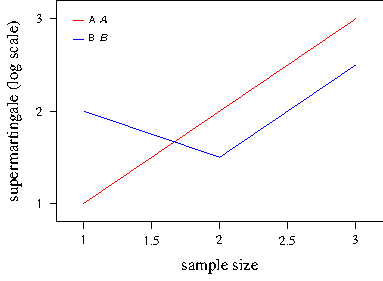
\includegraphics{scatterplot-tikz.pdf}
	\caption{TikZ, exact physical size, no scaling.}
\end{figure}

\begin{figure}[htb]
	\centering
	\begin{subfigure}[t]{2.8in}
		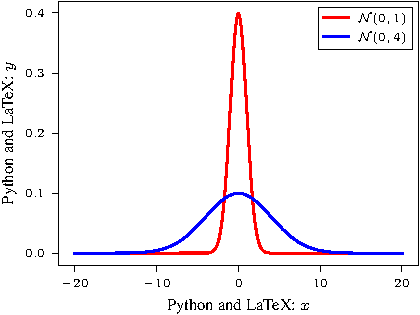
\includegraphics{scatterplot-python.pdf}
		\caption{Python $x$}
	\end{subfigure}\hfill
	\begin{subfigure}[t]{2.8in}
		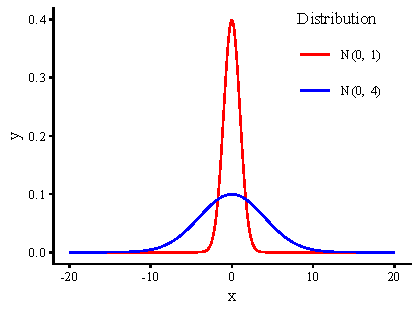
\includegraphics{scatterplot-R.pdf}
		\caption{R}
	\end{subfigure}

	\caption{Python vs R plots, exact physical size, no scaling.}
\end{figure}

\newpage
\section{Mathematical notation}

It has always been a hassle to organise mathematical notation across different sources,
in fact, I would go so far as to argue that this is the most annoying thing
when one starts reading a book or an article.

However, there \textit{must be} some notational conflicts beyond primary school
simply due to the fact that the limited number of alphabets (\textbf{26}).
For example, ``$\mathbb{E}$'' might be energy in physics
while it could refer to expectation or scores in probability.

Another difficulty is that the authors often assume some familiarity in the
topics
\emph{also} I am expected to read in some logical or chronological order.
In reality, I am constantly jumping back and forth between one literature to
another.

\begin{align*}
	\Af, \Bf, \Cf, \Df, \Ef, \Ff, \Gf, \Hf, \Jf, \Kf, \Lf, \Mf, \Nf, \Of, \Pf,
	\Qf, \Rf, \Sf, \Tf, \Uf, \Vf, \Wf, \Xf, \Yf, \Zf      \\
	\Ac, \Bc, \Cc, \Dc, \Ec, \Fc, \Gc, \Hc, \Ic, \Jc, \Kc, \Lc, \Mc, \Nc, \Oc,
	\Pc, \Qc, \Rc, \Sc, \Tc, \Uc, \Vc, \Wc, \Xc, \Yc, \Zc \\
	\Ak, \Bk, \Ck, \Dk, \Ek, \Fk, \Gk, \Hk, \Ik, \Jk, \Kk, \Lk, \Mk, \Nk, \Ok,
	\Pk, \Qk, \Rk, \Sk, \Tk, \Uk, \Vk, \Wk, \Xk, \Yk, \Zk
\end{align*}
$$
	\arginf, \argsup, \argmax, \argmin, \conv
$$

This stackexchange answer: \url{https://tex.stackexchange.com/a/58124}
is probably the most comprehensive answer to which fonts are shown in \LaTeX.

\begin{tabular}{ccl}
	\textbf{Symbol} & \textbf{Usage} & \textbf{Comments}                                 \\
	$\Bf$           & \verb|\*f|     & blackboard bold except \verb|\If| due to conflict \\
	$\Bc$           & \verb|\*c|     & calligraphic font                                 \\
	$\Bk$           & \verb|\*k|     & Fraktur font                                      \\
\end{tabular}

\subsection{Choose the notations and shortcuts wisely}

I am not even talking about the difference due to differences in fonts and italic or roman.
It is just a very sad thing that we don't even have a unified way of saying probability is just sad.
Take probability for example and return to the most basic case of tossing a
coin
where the sample space is $\Ac = \{H, T\}$. I have come across:

\begin{align*}
	P() \quad \mathrm{P}() \quad \mathrm{Pr}() \quad \mathsf{P}() \quad
	\mathbf{Prob}().
\end{align*}

\end{document}